\subsection{二次元要素と形状関数}
各要素の形状と節点配置を\cref{fig:2D_Element_Library}に示す.
三角形要素には面積座標(Area Coordinates)$L_i$ を,四角形要素には自然座標(Natural Coordinates)$(\xi, \eta)$ を適用する.
\begin{figure}[H]
  \centering
  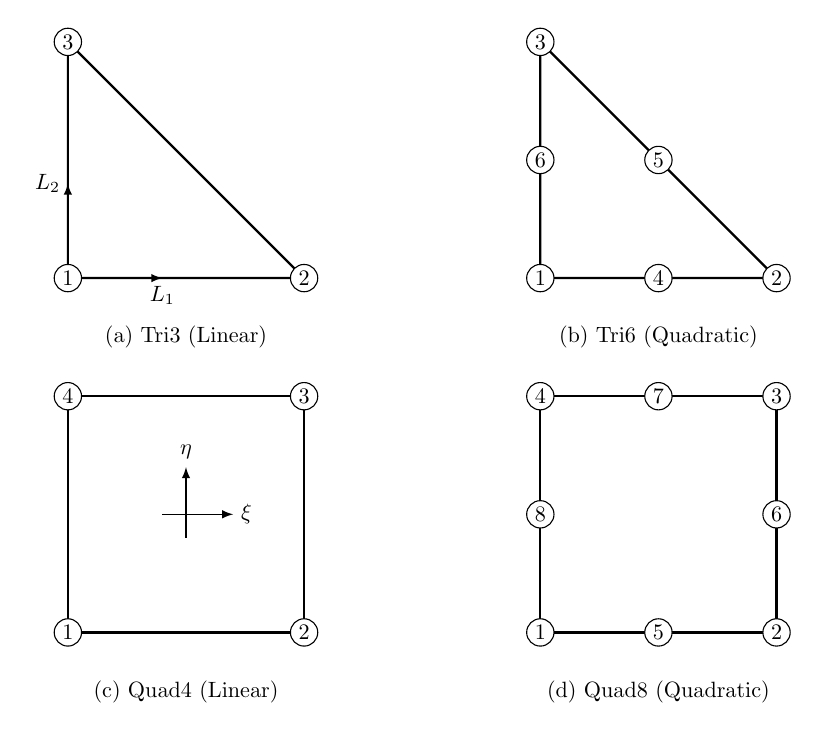
\begin{tikzpicture}[scale=1.5, every node/.style={scale=0.8}]
    % Define styles
    \tikzstyle{node_style}=[circle, draw, fill=white, inner sep=1.5pt]
    \tikzstyle{elem_edge}=[thick]

    % --- (a) Tri3 ---
    \begin{scope}[shift={(0,3)}]
      % Axis
      \draw[elem_edge] (0,0) -- (2,0) -- (0,2) -- cycle;
      \draw[-latex] (0,0) -- (0.8,0) node[below]{$L_1$};
      \draw[-latex] (0,0) -- (0,0.8) node[left]{$L_2$};
      \node[node_style] at (0,0) {1};
      \node[node_style] at (2,0) {2};
      \node[node_style] at (0,2) {3};
      \node at (1, -0.5) {(a) Tri3 (Linear)};
    \end{scope}

    % --- (b) Tri6 ---
    \begin{scope}[shift={(4,3)}]
      \draw[elem_edge] (0,0) -- (2,0) -- (0,2) -- cycle;
      \node[node_style] at (0,0) {1};
      \node[node_style] at (2,0) {2};
      \node[node_style] at (0,2) {3};
      \node[node_style] at (1,0) {4};
      \node[node_style] at (1,1) {5};
      \node[node_style] at (0,1) {6};
      \node at (1, -0.5) {(b) Tri6 (Quadratic)};
    \end{scope}

    % --- (c) Quad4 ---
    \begin{scope}[shift={(0,0)}]
      \draw[elem_edge] (0,0) -- (2,0) -- (2,2) -- (0,2) -- cycle;
      \node[node_style] at (0,0) {1};
      \node[node_style] at (2,0) {2};
      \node[node_style] at (2,2) {3};
      \node[node_style] at (0,2) {4};
      \node at (1, -0.5) {(c) Quad4 (Linear)};
      % Axis
      \draw[-latex] (0.8,1) -- (1.4,1) node[right]{$\xi$};
      \draw[-latex] (1,0.8) -- (1,1.4) node[above]{$\eta$};
    \end{scope}

    % --- (d) Quad8 ---
    \begin{scope}[shift={(4,0)}]
      \draw[elem_edge] (0,0) -- (2,0) -- (2,2) -- (0,2) -- cycle;
      \node[node_style] at (0,0) {1};
      \node[node_style] at (2,0) {2};
      \node[node_style] at (2,2) {3};
      \node[node_style] at (0,2) {4};
      \node[node_style] at (1,0) {5};
      \node[node_style] at (2,1) {6};
      \node[node_style] at (1,2) {7};
      \node[node_style] at (0,1) {8};
      \node at (1, -0.5) {(d) Quad8 (Quadratic)};
    \end{scope}
  \end{tikzpicture}
  \caption{2次元アイソパラメトリック要素}\label{fig:2D_Element_Library}
\end{figure}

\subsubsection{三角形要素群 (Triangular Elements)}
三角形要素では面積座標 $L_1, L_2, L_3$ を用いる.これらは $L_1+L_2+L_3=1$ を満たすため,独立変数は2つ(例: $L_1, L_2$)となる.
一般の直交正規化座標 $(\xi, \eta)$ との対応は,通常 $\xi = L_1, \eta = L_2$ と置かれる.

\begin{description}
  \item[一次三角形要素 (Tri3)]
        線形補間を行う最も基本的な要素である.
        \begin{equation}
          \psi_1 = L_1, \quad \psi_2 = L_2, \quad \psi_3 = L_3
        \end{equation}
  \item[二次三角形要素 (Tri6)]
        各辺の中点に節点を追加し,物理量の二次分布を表現可能とした要素である.
        \begin{align}
          \text{頂点節点:} & \quad \psi_1 = L_1(2L_1-1), \quad \psi_2 = L_2(2L_2-1), \quad \psi_3 = L_3(2L_3-1) \notag \\
          \text{中間節点:} & \quad \psi_4 = 4L_1L_2, \qquad~~ \psi_5 = 4L_2L_3, \qquad~~ \psi_6 = 4L_3L_1
        \end{align}
\end{description}

\subsubsection{四角形要素群 (Quadrilateral Elements)}
四角形要素では,正規化座標 $(\xi, \eta) \in [-1, 1] \times [-1, 1]$ を用いる.

\begin{description}
  \item[一次四角形要素 (Quad4)]
        双一次(Bilinear)補間を行う要素である.
        \begin{equation}
          \psi_i = \frac{1}{4}(1 + \xi_i \xi)(1 + \eta_i \eta) \quad (i=1,\dots,4)
        \end{equation}
        ここで $(\xi_i, \eta_i)$ は各節点の正規化座標である.
  \item[二次四角形要素 (Quad8)]
        各辺の中点に節点を追加したSerendipity族の二次要素である.中心節点を持たないため計算効率が良い.
        \begin{align}
          \text{隅節点 ($i=1\dots4$):} & \quad \psi_i = \frac{1}{4}(1 + \xi_i \xi)(1 + \eta_i \eta)(\xi_i \xi + \eta_i \eta - 1) \notag \\
          \text{中間節点 ($\xi_i=0$):}  & \quad \psi_i = \frac{1}{2}(1 - \xi^2)(1 + \eta_i \eta) \notag                                  \\
          \text{中間節点 ($\eta_i=0$):} & \quad \psi_i = \frac{1}{2}(1 + \xi_i \xi)(1 - \eta^2)
        \end{align}
\end{description}

\subsection{数値積分の統一的扱い}
剛性行列や質量行列の算出に必要な要素領域積分は,Gauss-Legendre積分公式を用いて次のように統一的に記述される.

\begin{equation}
  \label{Eq:Unified_Integration}
  \iint_{\Omega^e} F(\vect{x}) \odif{x}\odif{y} = \sum_{p=1}^{N_\mathrm{int}} w_p F(\xi_p, \eta_p) \det \mat{J}(\xi_p, \eta_p)
\end{equation}

ここで,$N_\mathrm{int}$ は積分点数,$w_p$ は重み係数,$(\xi_p, \eta_p)$ は積分点座標である.要素タイプごとの積分規則は以下の通りである.

\begin{table}[H]
  \centering
  \caption{各要素タイプにおける標準的な数値積分則}
  \label{Tab:Integration_Rules}
  \begin{tabular}{lcccc} \toprule
    \textbf{要素} & \textbf{座標系} & \textbf{積分点数}     & \textbf{積分次数} & \textbf{備考} \\ \midrule
    Tri3        & 面積座標         & 1点                & $O(h)$        & 重心積分        \\
    Tri6        & 面積座標         & 3点                & $O(h^2)$      & 辺の中点など      \\
    Quad4       & $\xi-\eta$   & $2 \times 2 = 4$点 & $O(h^2)$      & フル積分        \\
    Quad8       & $\xi-\eta$   & $3 \times 3 = 9$点 & $O(h^3)$      & フル積分        \\ \bottomrule
  \end{tabular}
\end{table}

なお,Quad8においては,計算コスト削減やロッキング回避のために低減積分($2 \times 2$点)が用いられる場合もある.